\documentclass[conference,a4paper]{IEEEtran}

\usepackage{amsmath,amssymb,amsfonts}
\usepackage{graphicx}
\usepackage{booktabs}
\usepackage{array}
\usepackage{textcomp}
\usepackage{xcolor}
\usepackage{microtype}
\usepackage{tikz}
\usetikzlibrary{shapes.geometric, arrows.meta, positioning}
\usepackage[colorlinks=true, linkcolor=black, citecolor=black, urlcolor=blue]{hyperref}

% ---- Diagram palette (figures only; tables/text stay plain IEEE black) ----
\definecolor{softblue}{RGB}{91,155,213}
\definecolor{softred}{RGB}{237,125,113}
\definecolor{softgreen}{RGB}{169,209,142}
\definecolor{softyellow}{RGB}{255,217,102}

\renewcommand{\arraystretch}{1.2}

\begin{document}

\title{Autotune in RTL: A Cycle-Accurate Phase-Vocoder Pitch-Shifting Datapath}

\author{
\IEEEauthorblockN{Rohan Jain, Dhananjay Dhumal, Gadgil Rucha Vinay, Karan Hitesh Bagthariya }
\IEEEauthorblockA{
Department of Electrical Engineering \\
Indian Institute of Technology Indore \\
Roll No.: 240002060, 240051008, 240002025, 240002028
}
}

\maketitle

\begin{abstract}
The purpose of this report is to describe the design, implementation, and verification of the RTL datapath for
an FPGA-based autotune engine using the Phase Vocoder algorithm. The third through tenth steps of a
twelve-step pitch-correction pipeline --- forward FFT, magnitude/phase conversion, pitch detection using a
tuning table, magnitude resampling, spectral reconstruction, and inverse FFT --- have been implemented as a
Vivado IP Integrator block design using Xilinx LogiCORE FFT and CORDIC IP along with Verilog control
logic, and have been structurally verified in the Vivado XSIM simulator and numerically compared with an
independent Python/NumPy reference model. This report describes the resulting architecture, the
verification process and results, a brutally honest account of the simplifications and challenges that arose
during implementation, and the next steps towards the ultimate goal of FPGA-based live-microphone
\end{abstract}

\begin{IEEEkeywords}
phase vocoder, pitch shifting, FPGA, FFT, CORDIC, Vivado, digital signal processing, autotune
\end{IEEEkeywords}

\section{Introduction}
Changing the frequency without changing the speed of an audio signal is done through frequency domain processing rather than time-domain resampling. This project builds the datapath of the \textbf{phase vocoder} autotune engine according to the twelve steps defined in the project specification: Ingestion, Windowing, FFT, Magnitude/Phase Conversion, Pitch Detection, Ratio calculation using the tuning table, Magnitude Resampling, Phase processing, Reconstruction, IFFT, Overlap-Add and Export.

In terms of the project scope, the \textbf{RTL deliverable involves the processing of Steps 3--10} (Transform through Inverse Transform) for one $N = 1024$ samples window, fully implemented in synthesizable Verilog through Xilinx Vivado IP Integrator. This report describes what has been delivered and proven through simulation in the \texttt{RTL Part} Vivado project, including those parts of the specification that have been simplified, replaced with another implementation approach, or postponed to a future version.

The autotune datapath is the deliverable for this project; however, it is also the initial step
in achieving a long-term objective: capturing \textbf{audio in continuous form via a live
microphone and running autotune on this audio using an FPGA}. The path to this objective is
described in Section~\ref{sec:future}, along with some platform directions the team is
exploring in parallel.

Table~\ref{tab:status} summarizes the status of each major deliverable at the time of
writing.

\begin{table*}[!t]
\centering
\caption{Project Deliverable Status at a Glance}
\label{tab:status}
\begin{tabular}{p{4.2cm}p{2.6cm}p{9.8cm}}
\toprule
\textbf{Spec. Item} & \textbf{Status} & \textbf{Notes} \\
\midrule
Core RTL datapath (Steps 3--10) & Implemented and simulated & Built as a Vivado IP-Integrator block design, \texttt{design\_1} \\
Overlap-Add (Step 11) & Implemented & \texttt{ifft\_ola} module (Section~\ref{sec:arch}) \\
Python golden-model cross-check & Implemented & Stage-by-stage NumPy reference compared against Vivado XSIM output; see Section~\ref{sec:verif} \\
Input stimulus generation & Implemented in Python & \texttt{AutotuneRTLProject.ipynb}; see Section~\ref{sec:verif} \\
Audio egress (FIFO + output handshake) & \textbf{Deferred} & Implemented in RTL but not yet wired into the verified pipeline; see Section~\ref{sec:future} \\
Cross-frame phase unwrapping (Step 8) & \textbf{Partially implemented} & Single-window scope; see Section~\ref{sec:limitations} \\
\bottomrule
\end{tabular}
\end{table*}

The remainder of this report is organized as follows. Section~\ref{sec:arch} describes the
system architecture. Section~\ref{sec:impl} details the module-level implementation.
Section~\ref{sec:dataformats} documents the data formats used across the pipeline.
Section~\ref{sec:verif} presents the verification methodology and results.
Section~\ref{sec:limitations} records known issues and simplifications.
Section~\ref{sec:future} outlines future work, and Section~\ref{sec:conclusion} concludes
the report.

\section{System Architecture}
\label{sec:arch}
The datapath is constructed in a block design (\texttt{design\_1.bd})
that connects four Xilinx LogiCORE IP blocks (two of Fast Fourier Transform cores and two of
CORDIC cores, with a clocking wizard) and six custom Verilog control/adapter modules
(\texttt{mem\_reader}, \texttt{fft\_config}, \texttt{spectral\_analysis},
\texttt{spectral\_transform}, \texttt{spectrum\_to\_cordic}, \texttt{ifft\_config}),
with the final module being the overlap-add block (\texttt{ifft\_ola}) in AXI4-Stream.
The full signal chain currently implemented and verified can be seen in Fig.~\ref{fig:pipeline}.
As stated in Table~\ref{tab:status} and explained in Section~\ref{sec:future},
the audio-egress block (a Block-RAM FIFO and an output handshake module) has already been
designed but is deliberately excluded from the pipeline at this point of time.

\begin{figure*}[!t]
\centering
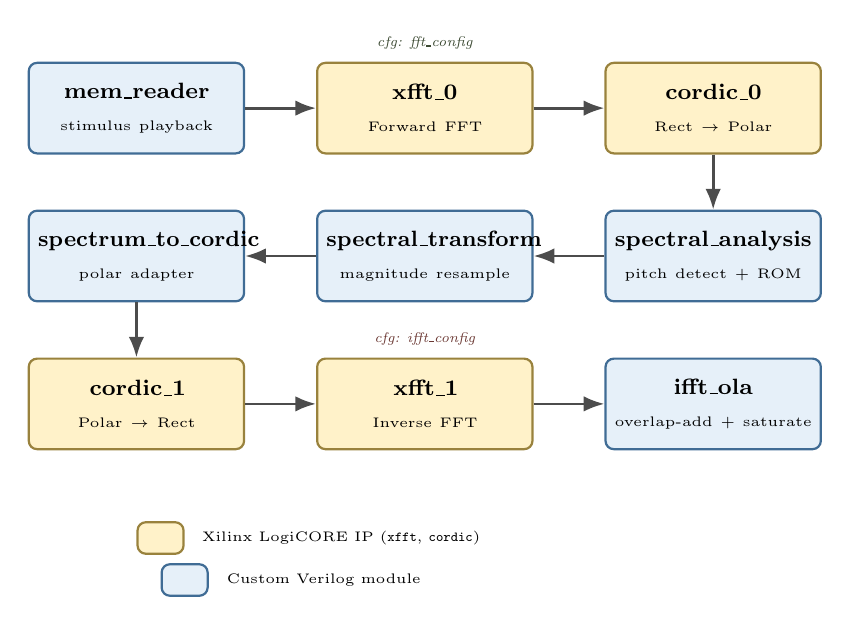
\begin{tikzpicture}[
    node distance = 0.7cm and 0.9cm,
    every node/.style={font=\footnotesize},
    blk/.style={draw=softblue!70!black, fill=softblue!15, rounded corners=3pt, align=center,
                text width=2.5cm, minimum height=1.15cm, line width=0.8pt},
    ipblk/.style={blk, fill=softyellow!35, draw=softyellow!60!black},
    line/.style={draw=black!70, -Latex, line width=1pt}
]

% -------- Row 1 (left to right): frame in -> forward FFT -> magnitude/phase --------
\node[blk]                   (mem)      {\textbf{mem\_reader}\\[2pt]{\tiny stimulus playback}};
\node[ipblk, right=of mem]   (xfft0)    {\textbf{xfft\_0}\\[2pt]{\tiny Forward FFT}};
\node[ipblk, right=of xfft0] (cordic0)  {\textbf{cordic\_0}\\[2pt]{\tiny Rect $\to$ Polar}};

% -------- Row 2 (right to left): pitch detect -> ratio -> resample -> adapt --------
\node[blk, below=of cordic0]  (analysis)  {\textbf{spectral\_analysis}\\[2pt]{\tiny pitch detect + ROM}};
\node[blk, left=of analysis]  (transform) {\textbf{spectral\_transform}\\[2pt]{\tiny magnitude resample}};
\node[blk, left=of transform] (s2c)       {\textbf{spectrum\_to\_cordic}\\[2pt]{\tiny polar adapter}};

% -------- Row 3 (left to right): reconstruct -> inverse FFT -> overlap-add --------
\node[ipblk, below=of s2c]     (cordic1) {\textbf{cordic\_1}\\[2pt]{\tiny Polar $\to$ Rect}};
\node[ipblk, right=of cordic1] (xfft1)   {\textbf{xfft\_1}\\[2pt]{\tiny Inverse FFT}};
\node[blk, right=of xfft1]     (ola)     {\textbf{ifft\_ola}\\[2pt]{\tiny overlap-add + saturate}};

% -------- Sequential flow --------
\draw[line] (mem) -- (xfft0);
\draw[line] (xfft0) -- (cordic0);
\draw[line] (cordic0.south) -- (analysis.north);
\draw[line] (analysis) -- (transform);
\draw[line] (transform) -- (s2c);
\draw[line] (s2c.south) -- (cordic1.north);
\draw[line] (cordic1) -- (xfft1);
\draw[line] (xfft1) -- (ola);

% -------- Config-word annotations --------
\node[font=\tiny\itshape, text=softgreen!35!black, above=1pt of xfft0] {cfg: fft\_config};
\node[font=\tiny\itshape, text=softred!45!black, above=1pt of xfft1] {cfg: ifft\_config};

% -------- Legend (placed below the whole diagram) --------
\node[ipblk, minimum height=0.4cm, minimum width=0.4cm, text width=0.35cm,
      below=0.9cm of cordic1, anchor=north west] (legendip) {};
\node[right=3pt of legendip, font=\tiny, align=left, text width=4.6cm]
      {Xilinx LogiCORE IP (\texttt{xfft}, \texttt{cordic})};
\node[blk, minimum height=0.4cm, minimum width=0.4cm, text width=0.35cm,
      below=3pt of legendip, anchor=north west] (legendrtl) {};
\node[right=3pt of legendrtl, font=\tiny, align=left, text width=4.6cm]
      {Custom Verilog module};

\end{tikzpicture}
\caption{Current implementation of signal processing chain implemented and validated in
\texttt{design\_1.bd}, shown as serpentine process chain: Row~1 reads a frame and calculates
its forward transform; Row~2 does pitch detection, tuning-ROM read, and resamples magnitudes;
Row~3 creates the transformed signal, inverse transforms it and overlap-adds it to time
domain. Yellow boxes represent Xilinx LogiCORE IP cores; blue boxes are Verilog designs.}
\label{fig:pipeline}
\end{figure*}

All blocks run from a single \texttt{clk\_wiz\_0} (Clocking Wizard) output configured for a
100~MHz input and a 100~MHz output --- i.e.\ it is used purely as a buffered system clock
rather than for frequency translation in the current design.

% ============================================================
% PLACEHOLDER FIGURE 1 of 2.
% Replace the tikzpicture box below with:
%   \includegraphics[width=\linewidth]{block_design.png}
% once you have exported a screenshot of the Vivado IP Integrator
% canvas (Window > Block Design > Diagram, then Export as image).
% ============================================================
\begin{figure}[!t]
\centering

\includegraphics[width=\linewidth]{Block Diagram.png}
\caption{Vivado IP Integrator block-design canvas for \texttt{design\_1.bd}.}
\label{fig:blockdesign}
\end{figure}

\section{Module-Level Implementation}
\label{sec:impl}

\subsection{Frame Ingestion --- \texttt{mem\_reader}}
Rather than implementing the file/windowing front end in RTL (Steps 1--2 were explicitly
placed outside the RTL scope by the specification), \texttt{mem\_reader.v} plays back a
pre-computed sample array from a \texttt{.mem} file straight onto an AXI4-Stream master
interface. Each cycle it presents one complex sample with the imaginary part hard-wired to
zero, and asserts \texttt{TLAST} on the last sample of every \texttt{FRAME\_SIZE} block so
that downstream cores can detect frame boundaries. As instantiated in \texttt{design\_1},
it is parameterized for \texttt{SAMPLE\_WIDTH=16}, \texttt{FRAME\_SIZE=1024},
\texttt{NUM\_SAMPLES=1{,}000{,}000}, reading from \texttt{harmonic.mem}. All stimulus files
(\texttt{harmonic.mem}, a four-tone composite test signal at bins 40/100/180/250;
\texttt{sine\_test.mem}, a single bin-aligned tone; and \texttt{audio\_frames.mem}, real
speech windowed and framed from \texttt{sample-speech-1m.wav}) were generated in Python
rather than by hand --- see Section~\ref{sec:verif} for how.

\subsection{Forward Transform --- \texttt{xfft\_0} + \texttt{fft\_config}}
The FFT itself (Block A) is not hand-written; it uses the Xilinx \textbf{LogiCORE FFT
v9.1} IP, configured for a fixed $N=1024$-point transform, \texttt{pipelined\_streaming\_io}
architecture, 16-bit fixed-point data, a 16-bit phase-factor width, natural output ordering,
and LUT-based butterflies. The small custom module \texttt{fft\_config.v} drives the
core's AXI4-Stream configuration channel once per reset with the constant word
\texttt{16'h0555}, which selects \texttt{FWD\_INV=1} (forward transform) and a fixed scaling
schedule (\texttt{1010101010}) chosen to keep the output in range for $N=1024$ without an
explicit block-floating-point stage.

\subsection{Rectangular-to-Polar Conversion --- \texttt{cordic\_0}}
Block B (Conversion of Magnitude/Phase, Step 4) is fully implemented using the
Xilinx \textbf{CORDIC v6.0} IP core instead of writing custom logic for square root and arctangent.
The core \texttt{cordic\_0} is instantiated to perform the \textit{Translate} operation (from rectangular
coordinates to polar coordinates), with data in signed-fraction format, compensation by
LUT scaling, and nearest even rounding, receiving the complex output $a+jb$ from the FFT.

\subsection{Pitch Detection and Ratio Calculation --- \texttt{spectral\_analysis}}
This is the largest hand-written block and implements Steps 5--6 (Pitch Detection, Ratio
Calculation) as a seven-state FSM (\texttt{RECEIVE} $\to$ \texttt{FREQ} $\to$ \texttt{ROM}
$\to$ \texttt{RATIO} $\to$ \texttt{DONE\_PULSE} $\to$ \texttt{STREAM} $\to$ \texttt{WAIT}):
\begin{itemize}
    \item \textbf{Capture:} the full 1024-bin magnitude/phase spectrum from \texttt{cordic\_0}
    is latched into two on-chip arrays (\texttt{magnitude\_mem}, \texttt{phase\_mem}).
    \item \textbf{Peak detection:} in the same pass, a running-maximum comparator tracks the
    largest-magnitude bin, explicitly excluding the DC bin (bin 0) and the
    negative-frequency mirror (bins $\geq N/2$), so only a genuine positive-frequency peak
    can win.
    \item \textbf{Frequency estimate:} \texttt{detected\_freq = peak\_bin} $\times$
    \texttt{SAMPLE\_RATE} $/$ \texttt{FRAME\_SIZE} (default \texttt{SAMPLE\_RATE = 44100~Hz}).
    \item \textbf{Tuning ROM search:} an 88-entry ROM (\texttt{tuning\_rom.mem}), holding the
    equal-tempered frequency of every piano key from A0 (28~Hz) upward as 16-bit hex values,
    is scanned linearly (one entry per clock) for the closest note to the detected frequency.
    \item \textbf{Ratio:} the pitch-shift factor is produced in \textbf{Q16.16} fixed point as
    \texttt{shift\_ratio = (closest\_frequency << 16) / detected\_freq}, defaulting to unity
    (65536, i.e.\ $S=1.0$) when no frequency is detected (silence/DC).
    \item The captured spectrum is then re-streamed out to \texttt{spectral\_transform} while
    the block waits for that stage to finish before accepting the next frame.
\end{itemize}

\subsection{Magnitude Resampling --- \texttt{spectral\_transform}}
This module implements Step 7 (and, in a simplified form, Step 9). For every output
(``target'') bin it computes the corresponding source bin as
\[
    \text{source\_bin} = \left\lfloor \frac{\text{target\_bin}}{S} \right\rfloor,
    \qquad S = \frac{\text{shift\_ratio}}{2^{16}},
\]
implemented with a single 64-bit fixed-point division
(\texttt{(target\_bin << 16) / shift\_ratio}), and copies that source bin's magnitude and
phase into the target bin. The DC bin and Nyquist bin are passed through unchanged, and the
negative-frequency half of the spectrum ($N/2 < k < N$) is regenerated from the positive
half by conjugate (Hermitian) symmetry, i.e.\ magnitude mirrored and phase negated, exactly
as required for a real-valued time-domain result after the inverse transform.

\textbf{Notes on Fidelity:} the specification's worked example makes use of \
\textit{linear interpolation} of two adjacent magnitude bins with fractional weight $F$
(\ $\text{Mag}_{\text{new}} = \text{Mag}_{10}(1-F) + \text{Mag}_{11}F$\ ).
However, the implemented RTL does \textbf{nearest-neighbour (floor) resampling}, which involves
taking the integer portion of the input index and discarding the fractional weight \
altogether. It was a design choice to simplify implementation and avoid an additional
per-bin multiply-accumulate step due to project time constraints; however, it leads to
slightly cruder spectral envelopes being generated than linear interpolation. See
Section~\ref{sec:limitations}.

\subsection{Polar-to-Rectangular Reconstruction --- \texttt{spectrum\_to\_cordic} + \texttt{cordic\_1}}
In Step 9 (Reconstruction), the same CORDIC IP family is employed in the reverse direction,
instead of doing a multiplication of $\text{mag}\cdot\cos(\phi) + j\,\text{mag}\cdot\sin(\phi)$.
The small converter \texttt{spectrum\_to\_cordic.v} takes the packed \{phase, magnitude\}
spectrum word and generates two streams: the Cartesian stream (magnitude is in the real part,
imaginary part is zero) and the phase stream, both going to \texttt{cordic\_1} that operates
in the \textit{Rotate} mode (polar to rectangular), thereby performing the reconstruction job
and outputting a true $a+jb$ complex number sample

\subsection{Inverse Transform --- \texttt{xfft\_1} + \texttt{ifft\_config}}
Step 10 utilizes a second occurrence of the same LogiCORE FFT IP (\texttt{xfft\_1}, the same 1024-point/16-bit/pipelined-streaming setup as \texttt{xfft\_0}), and \texttt{ifft\_config.v} is meant to configure it using \texttt{16'h0554} (\texttt{FWD\_INV=0}, inverse transformation). \textbf{This connection is not currently working for the block design} ---
Section~\ref{sec:limitations}.

\subsection{Overlap-Add --- \texttt{ifft\_ola}}
The implementation of step 11 is done in \texttt{ifft\_ola.v}. The 16 bit IFFT real sample is
extended to 18 bits and is added to the stored second half of the \emph{previous} frame (a 512 sample overlap memory,
that is, a 50\% overlap/\texttt{HOP\_SIZE = FRAME\_SIZE/2} hop approach --- unlike the 75\% overlap in the illustrative 
specification diagram). Then the 18 bit result is saturated to get back to 16 bit PCM. This is the final step of the verified 
pipeline; the output ports of this module (\texttt{fifo\_din}/\texttt{fifo\_wr\_en}) have been set up to feed a downstream FIFO,
though this FIFO and its audio-output-handshaking have been deliberately left unwired --- see
Section~\ref{sec:future}.

\section{Data Formats and Interfacing}
\label{sec:dataformats}
Every stage communicates over AXI4-Stream, and the same 32-bit packing convention is reused
throughout the design so that adjacent blocks agree on bit layout without extra glue logic,
as summarized in Table~\ref{tab:dataformats}.

\begin{table*}[!t]
\centering
\caption{AXI4-Stream Bit-Field Conventions}
\label{tab:dataformats}
\begin{tabular}{p{5.5cm}p{2.8cm}p{7.8cm}}
\toprule
\textbf{Interface} & \textbf{Bit Field} & \textbf{Meaning} \\
\midrule
mem\_reader $\to$ xfft\_0 & [31:16] / [15:0] & Imaginary / Real (16-bit signed, Q1.15) \\
cordic\_0 output & [31:16] / [15:0] & Phase (radians) / Magnitude (16-bit) \\
spectral\_analysis / transform spectrum bus & [31:16] / [15:0] & Phase / Magnitude \\
shift\_ratio & 32-bit & Q16.16 fixed point; $65536 = 1.0\times$ \\
xfft\_1 output & [31:16] / [15:0] & Imaginary / Real (16-bit signed, Q1.15) \\
ifft\_ola output (pre-FIFO) & [15:0] & 16-bit signed PCM \\
\bottomrule
\end{tabular}
\end{table*}

\section{Verification and Simulation}
\label{sec:verif}
There were two independent legs of the verification process: (i) structural/streaming verification of the RTL using the Vivado XSIM simulator; and (ii) numerical cross-validation of the RTL on a per-step basis using an independent Python/NumPy reference implementation. Both the test stimuli inputs into the RTL, as well as the gold outputs, were generated by the same Jupyter Notebook,
\texttt{AutotuneRTLProject.ipynb}.

\subsection{Python Reference Model and Stimulus Generation}
Rather than hand-writing \texttt{.mem} stimulus files or trusting the RTL's own arithmetic
as its own reference, every input file consumed by \texttt{mem\_reader} and every ROM
consumed by \texttt{spectral\_analysis} was generated programmatically in Python
(NumPy / SciPy) from \texttt{AutotuneRTLProject.ipynb}:
\begin{itemize}
    \item \textbf{\texttt{tuning\_rom.mem}} --- all 88 equal-tempered piano-key frequencies
    (MIDI notes 21--108, $A4=440$~Hz) computed directly from $f = 440 \cdot
    2^{(m-69)/12}$ and rounded to the nearest Hz.
    \item \textbf{\texttt{harmonic.mem}} --- a four-tone composite test signal (bins 40, 100,
    180 and 250, with amplitudes 4000/3000/2500/2000 and phases $30^\circ$/$45^\circ$/$60^\circ$/$90^\circ$),
    chosen so that the resulting FFT has known, well-separated, non-trivial (non-zero-phase)
    peaks that are easy to locate in a Vivado waveform dump.
    \item \textbf{\texttt{sine\_test.mem}} --- a single bin-aligned sine tone, used for the
    unit-level \texttt{mem\_reader\_tb} framing/handshake check.
    \item \textbf{\texttt{audio\_frames.mem}} --- real speech from \texttt{sample-speech-1m.wav},
    converted to mono, normalized, split into 1024-sample frames at a 512-sample hop (50\%
    overlap), Hann-windowed (\texttt{np.hanning}), and quantized to signed Q1.15 --- i.e.\
    Steps 1--2 of the specification (Ingestion, Windowing) were carried out in Python to
    produce realistic RTL input, rather than in RTL itself.
\end{itemize}

\subsection{Vivado-vs-Python Cross-Verification}
For every stage of the datapath, the notebook independently computed the same operation in
floating point and wrote the expected result to its own \texttt{.mem} file, so that Vivado's
actual output could be diffed against it stage by stage rather than only inspected at the
very end:
\begin{itemize}
    \item \textbf{Forward FFT:} \texttt{np.fft.fft} on \texttt{harmonic.mem} produced
    \texttt{fft\_expected.mem}, scaled to the same 16-bit range as \texttt{xfft\_0}.
    \item \textbf{Rectangular-to-polar (CORDIC \#1):} the Python model computes ideal
    magnitude/phase from the FFT result, then applies an \emph{empirically fitted} scale
    factor (magnitude $\times\,0.05286$, phase $\times\,8192$) obtained by comparing several
    sample points of the notebook's floating-point magnitude against the corresponding value
    actually captured from \texttt{cordic\_0} in a Vivado run --- e.g.\ Vivado/Python ratios
    of $1501/28377\approx0.05289$, $1250/23648\approx0.05286$ and $1000/18918\approx0.05286$
    were used to fix the constant. This lets the same notebook cell reproduce the specific
    fixed-point scaling used by the CORDIC IP rather than only its ideal mathematical
    behaviour.
    \item \textbf{Pitch detection, ROM search and magnitude resampling:} the notebook
    re-implements the \texttt{spectral\_analysis}/\texttt{spectral\_transform} logic in
    Python (peak search over bins $1 \ldots N/2-1$, nearest-ROM-entry search, ratio
    calculation, bin remapping and Hermitian symmetry) to produce an expected transformed
    spectrum for the same input.
    \item \textbf{Polar-to-rectangular (CORDIC \#2) and inverse FFT:} the notebook applies
    $\text{real} = \text{mag}\cos\theta$, $\text{imag} = \text{mag}\sin\theta$ and then
    \texttt{np.fft.ifft}, using \emph{truncation} rounding (matching the Vivado core's
    configured rounding mode) and 16-bit saturation, to produce a golden
    \texttt{ifft\_output.mem}.
\end{itemize}
For the test waveform shown above, the numerical output of the Python reference for the IFFT and
the actual waveforms observed from \texttt{ifft\_output.mem} in the Vivado XSIM simulation
are in very good agreement, sample-for-sample (e.g.\ 8-9, 2-3 and 1-2 for the real parts of the
first few samples, usually off by less than one LSB from each other with a small imaginary
component of a few LSBs in the latter where the former is exactly real).
This is \textbf{agreement after calibration}, not bit-accurate matching --- the CORDIC scaling
factor above is empirically determined and not from the datasheet of the IP, hence should be
taken as an approximation rather than a formally verified constant.

% ============================================================
% PLACEHOLDER FIGURE 2 of 2.
% Replace the tikzpicture box below with:
%   \includegraphics[width=\linewidth]{xsim_waveform.png}
% once you have exported an XSIM waveform/console screenshot
% (e.g. the ifft_output.mem capture, or a Vivado waveform viewer
% shot of m_axis_data_tdata / TLAST around the IFFT stage).
% ============================================================
\begin{figure}[!t]
\centering

\includegraphics[width=\linewidth]{ifft_out.png}
\caption{Output waveform obtained after the IFFT stage.}
\label{fig:ifftout}
\end{figure}

\subsection{XSIM Testbenches}
Independently of the Python cross-check, three Verilog testbenches exercise the streaming
and handshaking behaviour of the RTL directly in XSIM, as summarized in
Table~\ref{tab:testbenches}.

\begin{table*}[!t]
\centering
\caption{XSIM Testbenches}
\label{tab:testbenches}
\begin{tabular}{p{3.8cm}p{11cm}p{1.3cm}}
\toprule
\textbf{Testbench} & \textbf{Purpose} & \textbf{Scope} \\
\midrule
\texttt{mem\_reader\_tb} & Drives \texttt{mem\_reader} with a back-pressured AXI4-Stream
consumer over 4096 samples from \texttt{sine\_test.mem}; self-checks that the imaginary
field stays zero and that \texttt{TLAST} lands on exactly every 1024th sample. & Unit \\
\texttt{design\_1\_wrapper\_tb} & Instantiates the full \texttt{design\_1\_wrapper}, applies
reset, then logs every valid sample on the top-level output AXI4-Stream port. & System \\
\texttt{testing\_designs\_tb} / \texttt{testing\_wrappers.v} & Full-chain run that captures
every IFFT-stage output word to \texttt{ifft\_output.mem} via \texttt{\$fdisplay}, logs
\texttt{TLAST}, and includes a 10~ms safety timeout in case \texttt{TLAST} never arrives. &
System \\
\bottomrule
\end{tabular}
\end{table*}

All three testbenches ran to completion (\texttt{\$finish}) without triggering their
internal error checks (no imaginary-field violations, no missing/unexpected \texttt{TLAST}
events, no timeout), confirming correct \emph{streaming and structural} behaviour (framing,
handshaking, back-pressure) of the datapath. Combined with the Python cross-check above,
this gives reasonable confidence in both the structural and the numerical behaviour of the
pipeline, with the specific caveats recorded in Section~\ref{sec:limitations}.

\section{Known Issues and Simplifications}
\label{sec:limitations}
In the interest of an accurate report, the following gaps between the specification, the
intended design, and the as-built RTL were identified while writing this document:

\begin{enumerate}
    \item \textbf{Inverse-FFT configuration is disconnected.} Block-design
netlist inspection clearly shows that the net carrying the AXI4-Stream configuration
word for \texttt{ifft\_config\_0} to \texttt{xfft\_1} (\texttt{s\_axis\_config\_tdata}/\texttt{tvalid})
lacks a driving signal --- Vivado's synthesis log even points this out with the warning
\texttt{"WARNING: [BD 41-166] Source port for the net ifft\_config\_0\_config\_tdata is
NULL! Connection will be grounded!"}. Therefore, at the moment, \texttt{xfft\_1} operates with
its default configuration from power-up, rather than being instructed to do an inverse transform,
until its \texttt{ifft\_config\_0} output pins are properly connected to \texttt{xfft\_1} in the block
design. This issue is pointed out specifically rather than brushed aside, and is the most important thing
for revision. 
\item \textbf{Magnitude resampling uses nearest neighbour sampling instead of
linear interpolation.} As described in Section~\ref{sec:impl}, \texttt{spectral\_transform} truncates the fractional component of the source bin index,
as opposed to interpolation between the two closest bins. This can be fixed by an additional bin fetch followed by Q-format multiplication-addition at the cost of one.
    \item \textbf{No cross-frame phase unwrapping.} Because the RTL datapath is scoped to a
    single $N$-sample window (per the project specification), \texttt{spectral\_transform}
    carries phase straight through from the selected source bin with no phase-deviation
    computation, $[-\pi,\pi]$ wrapping, or persistent accumulator across frames (Block D of
    the specification). Extending the design to a real streaming/multi-frame pipeline would
    require an additional phase-accumulator register bank per bin, retained across calls ---
    see Section~\ref{sec:future}.
    \item \textbf{Six source files are empty Vivado-generated stubs} that were superseded by
    the IP-Integrator approach and never filled in: \texttt{fft.v}, \texttt{conversion.v},
    \texttt{reconstruction.v}, \texttt{ifft.v}, \texttt{overlap-add.v}, \texttt{overlapadd.v},
    \texttt{fft\_test\_bd.v}, \texttt{fft\_test.v} and \texttt{tb\_test.v}. Their intended
    roles were ultimately filled by the \texttt{xfft}/\texttt{cordic} IP cores and by
    \texttt{ifft\_ola.v} respectively; they are listed here for completeness rather than
    silently omitted.
\end{enumerate}

\section{Future Work and Extended Vision}
\label{sec:future}

\subsection{Near-Term: Completing the Current Datapath}
\begin{itemize}
\item \textbf{Audio egress.} \texttt{fifo\_generator} ($4096\times16$-bit, common clock
    block RAM FIFO) and \texttt{audio\_output\_handler} (first word fall-through read
    side handshake, provides \texttt{audio\_sample}/\texttt{audio\_valid}/\texttt{audio\_ready})
    are already available in the repository and previously connected directly to
    \texttt{ifft\_ola}. These have been intentionally omitted from the pipeline design
    described in this report --- and Fig.~\ref{fig:pipeline} --- until the upstream
    numerical problems in Section~\ref{sec:limitations} are addressed; their reintroduction
    will happen in
\end{itemize}

\subsection{Toward Continuous, Multi-Frame Operation}
The current datapath handles only one window of $N = 1024$ at a time. Achieving the
\textbf{true goal of the project --- continuous autotuning of real-time audio input from
a microphone on an FPGA} --- would mean transforming it into a proper streaming datapath,
involving continuous phase accumulation for each bin within overlapping frames (finishing Block D / Step 8, which we postponed in
Section~\ref{sec:limitations}) as well as a streaming ADC instead of ROM-based \texttt{mem\_reader}
and a continuous output audio flow.

\subsection{Extended Vision: A Real-Time Multi-Algorithm DSP Platform}
Nevertheless, while autotune is still the main objective of this project, the group is considering
extending its application to developing
the same FFT/CORDIC datapath in a wider context of \textbf{Real-Time Multi-Algorithm DSP
Platform}: a platform that processes the incoming real-time signal (like the microphone
audio), providing a choice between different DSP algorithms working with it -- Low-Pass, High-Pass, Band-Pass and Notch filtering, equalization, frequency analysis via FFT, and adaptive noise
cancellation -- along with adjustable runtime parameters (frequency cutoffs, gain, etc.) and a graphic display of the signal before and after processing. The idea is to illustrate how different classical DSP algorithms could be implemented using the same real-time hardware platform, processing the signal at different stages using signal-processing approaches instead of machine-learning.

\section{Conclusion}
\label{sec:conclusion}
A Steps 3-10 phase vocoder pipeline up through overlap add was constructed using
Vivado IP-Integrator design consisting of two Xilinx FFT cores, two Xilinx CORDIC cores,
88-note tuning ROM, and six custom Verilog control/adapters. The design was validated in
two ways: XSIM test benches verify proper stream, frame and back pressure operation from
end to end, and an independent reference model written in Python and NumPy,
implemented in \texttt{AutotuneRTLProject.ipynb} (and generating all input stimuli for testing)
is used to validate the numeric output of each pipeline stage, demonstrating close (but
calibrated, not bit-by-bit exact) matching to the results generated in Vivado. The two open
items in particular are documented exactly in Section~\ref{sec:limitations} (the standalone
configuration network for the inverse FFT and the nearest-neighbor magnitude
resampling), and Section~\ref{sec:future} maps the route from here to the final goal of
real-time, live microphone autotune using FPGA, along with the general DSP platform
directions the team plans to take.

\end{document}
